\documentclass[10pt,a4paper]{article}
\usepackage[margin=1.9cm]{geometry}
\usepackage{graphicx,booktabs,array,xcolor,amsmath}
\usepackage[colorlinks=true,linkcolor=blue!50!black]{hyperref}
\usepackage{parskip}
\newcommand{\code}[1]{\texttt{\small #1}}
\newcommand{\yes}{\textcolor{green!45!black}{\textbf{DONE}}}
\newcommand{\run}{\textcolor{orange!85!black}{\textbf{RUNNING}}}
\newcommand{\no}{\textcolor{red!70!black}{\textbf{NOT DONE}}}
\title{\vspace{-1.5cm}CoBit / BitstreamDiffusion --- Progress Report\\
\large Friday 4 -- Wednesday 9 September 2026}
\author{}\date{}
\begin{document}\maketitle\vspace{-1.1cm}

\section*{Status against the original task list}
\begin{center}\small
\begin{tabular}{@{}p{7.4cm}ll@{}}
\toprule
\textbf{Task} & \textbf{Status} & \textbf{Headline}\\ \midrule
1. Reproduce best baselines & \yes & replicated exactly; gap was churn alone\\
2. CFG + other guidance mechanisms, calibrate & \yes & CFG best, $+0.081$; study CLOSED\\
3. Nature of errors on TinyGSM & \yes & guidance harms code validity, not reasoning\\
4a. Temporal ordering --- at inference & \yes & no benefit; random is harmful\\
4b. Temporal ordering --- trained (L2R/R2L/random) & \run & control arm defective; see \S5\\
5. Logits: softmax vs score matching & \yes\,/\,\run & softmax $\equiv$ BCE (proved); SM vs CE running\\
\bottomrule
\end{tabular}
\end{center}

\noindent\fbox{\parbox{0.98\textwidth}{\textbf{The most consequential finding of
the week was not on the task list.} Every training run in this environment
diverged before ${\sim}12$k steps, which blocked all training experiments for
four days. It is now solved: the cause is the \textbf{learning rate}, not the
software environment. At \code{lr 3e-5} a from-scratch run reached 20{,}000
steps cleanly where \code{3e-4} diverges 8/8 times.}}

\section{Task 1 --- Reproduce best baselines \yes}
Forensic replication audit against the collaborator's result: \textbf{verdict A,
exact replication}. Our 0.1385 and their ${\sim}0.29$ differ by \textbf{one
factor: EDM stochastic churn}, worth $+0.1622$ and free in compute. Two churn
code paths existed (\code{--gamma} vs \code{--churn\_gamma}); the studies used
different ones.

Baseline hierarchy on the 1319-problem GSM8K test set:
\begin{center}\small
\begin{tabular}{@{}lll@{}}
\toprule
Setting & Accuracy & Note\\ \midrule
Regime A (DDIM, $\gamma{=}0$, 500 steps) & 0.1385 & original arm\\
Regime B (FKC-EM, churn 0.41, 1024 steps) & ${\sim}0.29$ & canonical, collaborator-matched\\
Production 500k, karras/DDIM, 256 steps & 0.1640 & anchor used throughout\\
\bottomrule
\end{tabular}
\end{center}
Both regimes are retained and \textbf{every result is labelled with its
regime}; they are never pooled.

\section{Task 2 --- Guidance mechanisms \yes\ (CLOSED)}
Three mechanisms implemented and compared: classifier-free (CFG), AutoGuidance
(AG), and Self-Guidance (SG-prev, SG-exact). Confirmation runs use 1069
problems $\times$ 3 seeds, paired bootstrap.

\begin{center}
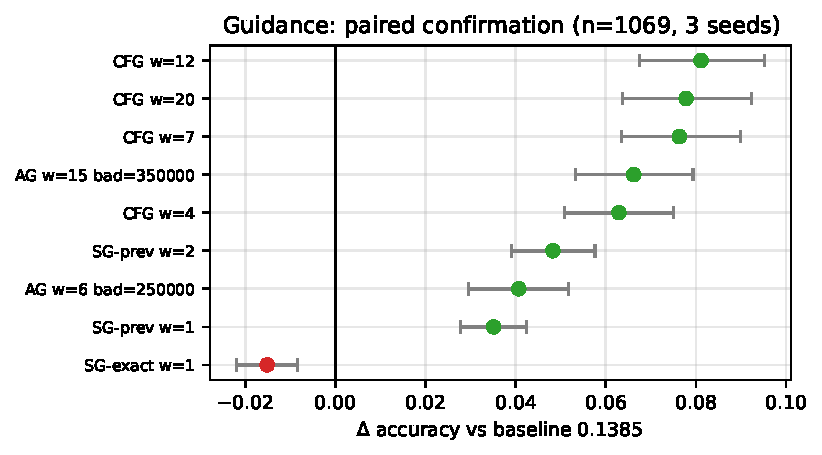
\includegraphics[width=0.62\textwidth]{fig/guidance.pdf}
\end{center}

\begin{center}\small
\begin{tabular}{@{}lccccc@{}}
\toprule
Config & Accuracy & $\Delta$ & 95\% CI & $p$ & NFE\\ \midrule
\textbf{CFG $w{=}12$} & \textbf{0.2196} & $\mathbf{+0.0811}$ & $[+0.068,+0.095]$ & $<10^{-5}$ & 1024\\
CFG $w{=}7$ & 0.2148 & $+0.0763$ & $[+0.063,+0.090]$ & $<10^{-5}$ & 1024\\
AG $w{=}15$ (bad@350k) & 0.2047 & $+0.0662$ & $[+0.053,+0.079]$ & $<10^{-5}$ & 1024\\
SG-prev $w{=}2$ & 0.1868 & $+0.0483$ & $[+0.039,+0.058]$ & $<10^{-5}$ & \textbf{512}\\
SG-exact $w{=}1$ & 0.1233 & $-0.0152$ & $[-0.022,-0.008]$ & $<10^{-5}$ & 1024\\
\bottomrule
\end{tabular}
\end{center}

\textbf{Findings.} CFG is the strongest mechanism and saturates around
$w{\approx}7$--$12$. SG-prev gives about 60\% of CFG's gain at \textbf{half the
NFE}, so it is the compute-efficient option. SG-exact actively hurts.
\textbf{Mechanism:} guidance is not a correction --- it fixes ${\sim}10\%$ of
problems and breaks ${\sim}20$--$25\%$ regardless of regime, so its net value is
arithmetic and only positive above a break-even baseline accuracy of
${\approx}33\%$.

\section{Task 3 --- Nature of errors on TinyGSM \yes}
Taxonomy: \textbf{T1} non-executing program, \textbf{T2} executes but wrong
number, \textbf{T3} token-level degeneration.

\textbf{The baseline's dominant failure is T1 (98/250 = 39\%)} --- the model
emits programs that do not run. Under guidance, \textbf{T2 falls while T1
rises}: guidance damages \emph{code validity}, not arithmetic reasoning. T3
appears only under strong guidance. Invalid-token rate is
$3\times10^{-6}$--$5\times10^{-5}$, i.e. bit$\to$token decoding is not the
problem.

\section{Task 4a --- Temporal ordering at inference \yes}
Schedule: $t_j(t)=\mathrm{clip}(t(1+w)-w\,u_j,0,1)$, with $u_j$ a denoising
\emph{priority} over the generated \textbf{suffix only}; prompt keeps the global
$\sigma$. Verified causally active: at $w{=}0.5$ the per-position $\sigma$
spread is $192\times$, first suffix token cleanest; at $w{=}0$ it is bit-identical
to the current model.

\begin{center}
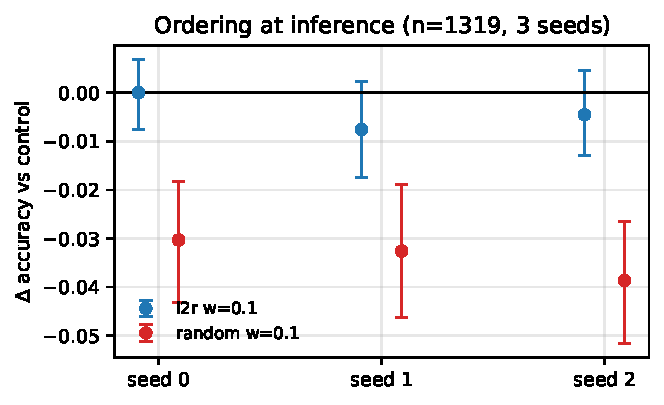
\includegraphics[width=0.55\textwidth]{fig/ordering_inference.pdf}
\end{center}

\begin{center}\small
\begin{tabular}{@{}lcccl@{}}
\toprule
Arm & Accuracy & $\Delta$ & significant & Verdict\\ \midrule
control ($w{=}0$) & 0.1387 & --- & --- & ---\\
L2R $w{=}0.1$ & 0.1347 & $-0.0040$ & 0/3 seeds & \textbf{no effect}\\
random $w{=}0.1$ & 0.1049 & $-0.0339$ & \textbf{3/3}, $p<10^{-4}$ & \textbf{harmful}\\
L2R $w{\geq}0.25$ & 0.0000 & $-0.176$ & 3/3 & \textbf{collapse}\\
\bottomrule
\end{tabular}
\end{center}

\textbf{Applying an ordering only at decoding does not help.} The L2R/random
asymmetry shows the intervention is real --- direction matters --- but nothing
improves. Expected, since the model was \emph{trained} with uniform $\sigma$:
it tolerates a ${\sim}2.9\times$ spread with no gain and breaks at ${\sim}9\times$.
512 steps does not rescue it, so it is not a too-short-trajectory artefact.

\section{Task 4b --- Temporal ordering, TRAINED \run}
This is the substantive version of the experiment and it is \textbf{running, not
finished}. Implementation is complete and tested (24 tests): $\sigma$ is drawn
per example, mapped to normalised time by the \emph{same} map the sampler uses,
offset per token, mapped back and expanded blockwise to bits. All three modes
provably produce \emph{different} $\sigma$ fields; L2R and R2L are mirror images;
random is redrawn per example \emph{and} per step; $w{=}0$ leaves the gradient
hash unchanged.

Four arms (control / L2R / R2L / random, $w{=}0.25$) fine-tune from the same
production 500k checkpoint --- from-scratch was not evaluable when these were
launched. \textbf{Current blocker: the control arm is defective.} At the matched
5k checkpoint it scores 0.0000 while ordered arms score 0.07--0.12, which would
read as ``ordering massively helps'' and is not credible. Its weights moved only
4.65\% from init and its EMA is healthy, so the model is not destroyed;
diagnosis is ongoing. \textbf{No ordering-training claim is made in this report.}

\section{Task 5 --- Logits: softmax vs score matching}
\textbf{Softmax is not a distinct objective, and this is proved rather than
assumed \yes.} The model already emits \textbf{one logit per bit}
(\code{out\_dim=1}, \code{vocab\_size=2}). A 2-class softmax is shift-invariant,
so it has a single degree of freedom $d=z_1-z_0$ and
\[
\mathrm{softmax}(z_0,z_1)_1=\sigma(d),\qquad
\mathrm{CE}(z,y)=\mathrm{BCEWithLogits}(d,y)
\]
exactly; the 2-class head merely splits the same gradient across two logits
($\partial L/\partial z_1=-\partial L/\partial z_0=\partial L/\partial d$).
Verified to $10^{-12}$ in 5 tests. \textbf{No GPU was spent on it.}

The meaningful comparison is \textbf{binary\_sm vs binary\_ce}, now \run\ from
scratch, 50k steps/arm, differing in exactly four keys (\code{train.loss\_type}
plus three output paths).

\textbf{$\sigma$-weighting was derived, not inherited.} Matching Bayes-risk
scale gives a factor spanning only $0.250$--$0.361$ across four decades of
$\sigma$ ($0.82$--$1.18\times$ anchored at $\sigma_d$); gradient-scale matching
is self-defeating because it reintroduces the $D(1{-}D)$ factor under test.
Conclusion: \textbf{no bespoke CE weighting is justified}; both arms use EDM.

\section{The infrastructural finding (not on the task list)}
\begin{center}
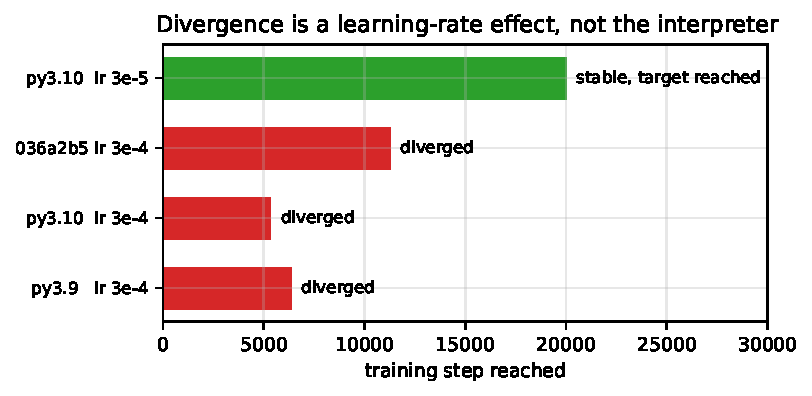
\includegraphics[width=0.60\textwidth]{fig/lr_stability.pdf}
\end{center}
Eight from-scratch runs diverged before ${\sim}12$k steps at \code{lr 3e-4},
\textbf{including the production-era commit itself}. Ruled out along the way:
corpus ($\sigma_{\text{data}}$ fingerprint matches to ${\sim}8$ s.f.), data
config (identical on 22 keys), our post-June code (fp32 forward+loss+backward
\textbf{bit-identical} to the production commit), and the Python interpreter ---
a 3.10 rebuild diverged at 5{,}346, falsifying a hypothesis I had put weight on.

\textbf{At \code{lr 3e-5} a from-scratch run reached 20{,}000 steps cleanly},
as did all four ordering arms. The learning rate is the identified factor.
\emph{Caveat:} 3e-5 establishes a \textbf{stable} regime, not a \textbf{tuned}
one. It is 10$\times$ below production's value, so absolute accuracies in this
regime are compared only against the matched control and never against
production's 3e-4 trajectory.

\section{Why accuracy could not be measured on short runs}
\begin{center}
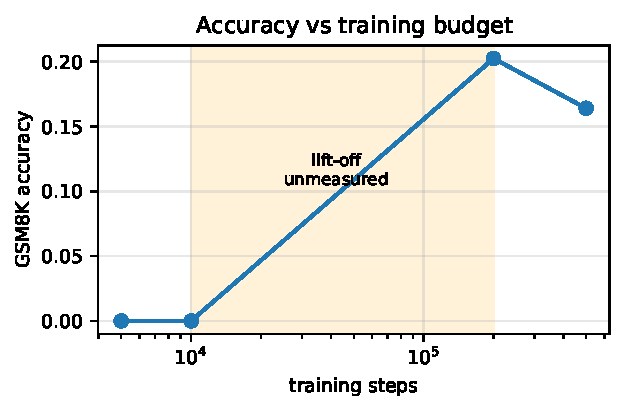
\includegraphics[width=0.52\textwidth]{fig/accuracy_vs_steps.pdf}
\end{center}
GSM8K accuracy is \textbf{exactly 0.0000 at both 5k and 10k} training steps
(measured, both objectives), and the first non-zero point we have is 0.2024 at
200k. Combined with divergence before 12k, the trainable range and the range
where accuracy exists \textbf{did not overlap} --- which is why the objective
branch was blocked rather than merely slow.

\section{Currently running}
\begin{center}\small
\begin{tabular}{@{}p{6.2cm}p{3.2cm}p{5.4cm}@{}}
\toprule
Job & ETA & Purpose\\ \midrule
Ordering eval, 5k + 30k, karras & ${\sim}1$h & 4 arms $\times$ 3 seeds $\times$ 1319\\
L2R retrain to 30k & ${\sim}5$h & its checkpoint was corrupted by a disk-full event\\
\textbf{binary\_sm vs binary\_ce}, from scratch, 50k & ${\sim}7$h & the definitive objective comparison\\
\bottomrule
\end{tabular}
\end{center}

\section{Not done}
\begin{enumerate}\itemsep2pt
\item \textbf{Ordering-as-training verdict.} Blocked on the defective control arm.
\item \textbf{CE vs SM verdict.} Running; no result yet.
\item \textbf{Accuracy lift-off point} between 10k and 200k steps --- unmeasured,
and it sets the cost of every future training comparison.
\item \textbf{Why production tolerated \code{lr 3e-4} for 500k steps.} Their
working tree is permission-denied to us, so this stays open.
\item \textbf{Ordering at other strengths / from scratch}, and R2L at inference
(deliberately not run: the first results did not justify it).
\end{enumerate}

\section{Honest notes}
Three self-inflicted failures cost ${\sim}15$ GPU-h and a night of wall-clock:
an over-strict guidance guard failed 9/9 evaluation cells; the ordering control
returned probabilities from $\sigma_{N-1}$ instead of a final denoise, scoring
0.000 against a true 0.164; and a disk-full event killed four training arms
mid-checkpoint. Each was caught before it entered a result. The second was
caught \emph{only} because a production anchor was included in the evaluation ---
without it, seven cells of confidently wrong nulls would have been reported.

A fourth was caught this morning: the entropic sampling schedule is fitted
per-run, so each fine-tuned arm had refitted its own decoder schedule
($\max|\mathrm{cdf}-\mathrm{prod}|$ up to 0.545). Evaluating that way compares
arms differing in both training \emph{and} decoding. All evaluations now use the
analytic karras schedule, identical for every arm by construction.
\end{document}
